\section{Introducción}

La \textbf{arquitectura de una computadora} es el conjunto de recursos accesibles para el programador que, por lo general, se mantienen a lo largo de los diferentes modelos de procesadores de esa arquitectura (puede evolucionar pero la tendencia es mantener compatibilidad hacia los modelos anteriores).

Diseñar una arquitectura implica diseñar las interfaces hardware/software para crear un sistema computacional que posea los requerimientos funcionales, de perfomance, consumo (de energía) y de costo (económico) adecuados para realizar determinadas tareas.

\begin{wrapfigure}{r}{0.5\textwidth}
	\centering
	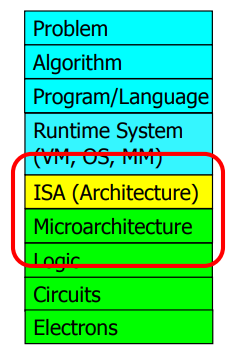
\includegraphics[width=0.25\textwidth]{imagenes/arquitectura}
	\caption{La computadora definida en niveles de abstracción}
	\label{fig:intro::arquitectura}
\end{wrapfigure}

Estas tareas son problemas que pasaron por varias transformaciones (desde su descripción en un lenguaje natural hasta convertirse en un programa) y deben ser ejecutadas por una computadora. La tarea del arquitecto consiste en diseñar el \textbf{Instruction Set Architecture} (ISA), un conjunto de instrucciones que usarán los programas compilados para decir al micropocesador que hacer. El ISA es implementado por un conjunto de estructuras de hardware conocidas como \textbf{microarquitectura}.

El ISA y la microarquitectura sientan las bases para que el diseño del procesador consiga el balance adecuado de los factores mencionados y pueda llevar a cabo ciertas tareas de la manera más optima posible. Habrá casos en los que daremos prioridad a un subconjunto de ellos en detrimento de otros (por ejemplo, podriamos elegir mejorar perfomance y aumentar el costo, o quitar performance para mejorar el consumo energético).

\subsection{Componentes del ISA}
El ISA es la especificación completa de la interfaz entre los programas y el hardware que debe llevar a cabo las operaciones. Entre otras cosas, especifica:

\subsubsection{Regitros}
\begin{itemize}
	\item \textbf{Registros:} Celdas de memoria dentro del cpu que son usadas para almacenar los datos necesarios para ejecutar una instrucción. Éstos, son visibles al programa y se clasifican según su uso: Acumuladores, De dirección ó De Proposito General.
	\item  \textbf{Instrucciones}: Tareas que pueden ser llevadas a cabo por la computadora. Cada una de ellas está compuesta por su \textbf{opcode} (que se espera que la computadora haga) y sus \textbf{operandos} (a que datos debe hacerlo). En una ISA podremos encontrar tres tipos de instrucciones:
	\begin{itemize}
		\item De \textbf{Operacion}: Procesan datos.
		\item De \textbf{trasnporte}: Transportan información entre la memoria, los registros y los dispositivos de entrada salida.
		\item De \textbf{control (Branching)}: Modifican la secuencia de instrucciones a ser ejecutada, es decir, permiten ejecutar instrucciones que no están almacenadas secuencialmente.
	\end{itemize}
	
	Dependiendo que valores puedan modificar las instrucciones de operación, podremos clasificar las arquitecturas en: \textbf{Arquitecturas Load/Store} (solo pueden operar en registros) o \textbf{Arquitecturas memory/memory} (se pueden modificar los valores directamente en memoria)
	\item \textbf{Tipos de datos}: Representación que deben tener ciertos valores para poder ser interpretados por la microarquitectura.
	\item \textbf{Espacio de memoria}: La cantidad de bloques univocamente distinguibles en memoria y el tamaño de cada uno de estos bloques
	\item \textbf{Direccionamiento}: Los mecanismos usados por la computadora para saber donde están almacenados los datos. Puede ser:
	\begin{itemize}
		\item \textbf{Inmediato:} El operando está incluido en la instrucción.
		\item \textbf{Directo o absoluto:} El operando es la dirección de memoria donde se encuentra el valor a ser utilizado.
		\item \textbf{Indirecto:} El operando es una dirección de memoria donde se encuentra la dirección de memoria en la que está almacenado el valor deseado.
		\item \textbf{De desplazamiento:} La instrucción toma como operandos una dirección de memoria que se toma como \textbf{base} y un \textbf{offset}. La base es una dirección de memoria y el offset, un número que indica cuanto hay que desplazar la base para encontrar el valor deseado, es decir $dir = base + offset$
		\item \textbf{Indexado:} Lo mismo que el anterior, pero con el \textit{offset} guardado en un registro.
		\item \textbf{De Memoria Indirecta:} El operando es un registro en el que se encuentra guardada la dirección de memoria indirecta.
	\end{itemize}
	\item \textbf{I/O Interface}: Como comunicarse con los dispositivos de entrada/salida. Puede ser por medio de instrucciones especiales o mapeos de ciertas regiones memoria para uso de esos dispositivos.
	\item \textbf{Modos de privilegio:} Quien puede y quien no puede ejecutar ciertas instrucciones 
	\item \textbf{Manejo de expcepciones e interrupciones:} Qué debe suceder si una instrucción falla o cuando un dispositivo necesita usar el microprocesador.
	\item \textbf{Soporte de memoria virtual:} Si soporta o no el uso de \textbf{memoria virtual}, es decir, si cada programa tiene la ilusión de estar un espacio de memoria secuencial cuando en realidad el sistema operativo realiza el manejo de la memoria principal.
\end{itemize}

\subsubsection{Arquitectura de Von Neumann}\label{sec::Intro::ISA::Von_Neuman}
Como se vió en Organización del computador I, las mayoría de las ISA usadas actualmente usan el modelo de Von Neumann. Éste es un ciclo de cuatro etapas: 

\begin{enumerate}
	\item \textbf{Fecth:} Se utiliza un \textbf{program counter} para saber donde está almacenada la proxima instrucción a ser ejecutada. Y se carga desde la memoria.
	\item \textbf{Decode:} Se decodifica la instrucción fetcheada y se consiguen los operandos (literales y registros) correspondientes.
	\item \textbf{Execute:} En esta etapa se busca en memoria los datos requeridos (si es necesario) y se procesa los datos acorde a la instrucción.
	\item \textbf{Write Back:} Se almacenan los resultados obtenidos en el lugar indicado.
\end{enumerate}

\begin{figure}[ht]
	\centering
	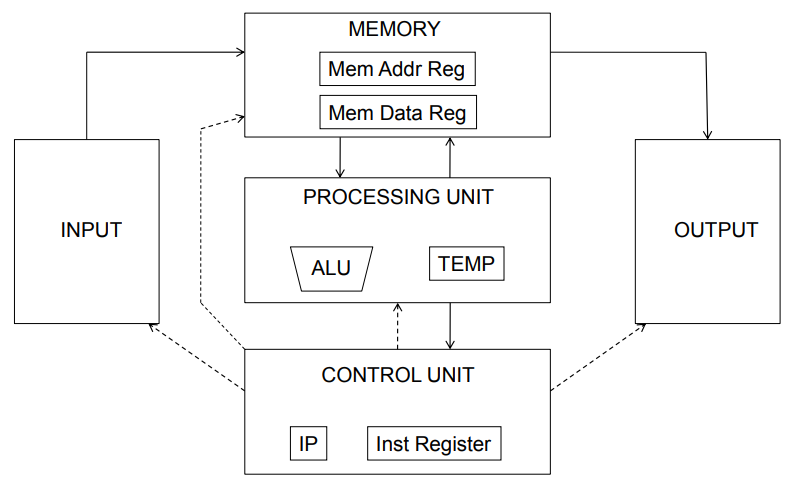
\includegraphics[width=0.4\textwidth]{imagenes/von-neuman-arquichtecture}
	\caption{Arquitectura de Von Newmman}
	\label{fig:intro:componentesIsa::vonsneumanarquichtecture}
\end{figure}
Cada instrucción es extraída de la memoria usando la dirección indicada por el \textbf{Instruction Pointer}. La unidad de control se encarga de indicar a la memoria si son necesarios otros valores para poder llevar a cabo su ejecución y, luego, pasa todo los datos a la unidad de procesamiento.

Si bien este es el ciclo que ``ve'' un programador, la implementación de las ISA (microarquitectura) usa estructuras de hardware más complejas que permiten acelerar la ejecución de cada fase.

\subsection{Microarquitectura}
La micoarquitectura es la implementación a nivel hardware de la ISA, es decir, es un conjunto de componentes electrónicos organizados de cierta manera para que respeten esas especificaciones.  Desde el punto de vista de la implementación (hardware), el ciclo es realizado por unidades de procesamiento que operan sobre los datos de acuerdo a ciertas señales. 

Cada instrucción es una señal que usa el procesador de instrucciones para decidir que conjunto de componentes electrónicos deben ser activados para poder llevar a cabo la operación deseada. Especificamente, las instrucciones indican: 

\begin{itemize}
	\item \textbf{Datapath:} Que elementos deben manejar y transformar los datos (unidades de procesamiento, de almacenamiento y estructuras de hardware que permiten el flujo de datos)
	\item \textbf{Control Logic:} Que elementos de hardware determinan las señales de control que indican al datapath lo que debe hacer con los datos.
\end{itemize}

En otras palabras, la microarquitectura comprende la tecnología utilizada para construir el hardware, la organización e interconexión de la memoria, el diseño de los bloques de CPU y la implementación de distintos mecanismos de procesamiento que no son visibles para el programador. 

%\subsection{Medidas de Performance}
%La escala y complejidad de los sistemas de software modernos, junto con las técnicas usadas por los diseñadores de hardware para mejorar el rendimiento de los dispositivos, ha logrado hacer que el rendimiento pueda depender de varios factores.
%
%\subsubsection{Response time}
%A veces, mediremos el rendimiento de una computadora en base a su tiempo de respuesta (\textbf{response time} o \textbf{execution time}) - el tiempo entre que pasa entre que una tarea empieza y termina -. Este tiempo se mide en segundos por programa y mide el tiempo total que toma completar una tarea, incluyendo accesos a memoria, operaciones del sistema, etc.
%
%En la práctica, la computadora es compartida por varios programas y los microprocesadores deben ejecutar varias tareas simultáneamente. En estos casos, deberemos tener en cuenta que la tarea que la tarea que se está evaluando, no está siendo ejecutada todo el tiempo por lo qué habrá que distinguir el tiempo que el procesador pasa ejecutando la tarea  \textbf{CPU Time} del tiempo en el que está procesando otros programas.
%
%Entonces, el tiempo de ejecución se define de la siguiente manera:
%
%$$Response~Time = \frac{Clock~Cycles~spent~on~task}{Clock~Rate}$$
%
%Donde \textit{Clock Cycle} son la cantidad de ciclos de reloj (ticks) que se utilizaron en la tarea y \textit{Clock Rate} es el tiempo que dura cada tick del reloj.
